\documentclass[preprint,12pt]{elsarticle}

\usepackage{amsmath}
\usepackage{amssymb}
\usepackage{amsthm}
\usepackage{graphicx}
\usepackage{subcaption}
\captionsetup{font=small,labelfont=bf}
\usepackage[section]{placeins}
\usepackage{booktabs}
\usepackage{algorithm}
\usepackage{algpseudocode}
\usepackage{siunitx}
%% Without this, the .bbl falls back to \texttt for URLs, which cannot break
%% and pushes two ScienceDirect links ~75pt past the right margin.
\usepackage{url}
\usepackage{tikz}
\usetikzlibrary{arrows.meta,positioning,fit,calc,backgrounds}
%% Shared palette for the TikZ schematics; frenetink matches the "ours" curve
%% colour of the result figures (see src/paper_style.py, COL["Frenet"]).
\definecolor{frenetink}{HTML}{3B33A0}
\definecolor{previewor}{HTML}{E8820C}
%% Without these the document falls back to bitmap (Type 3) EC fonts, which look
%% ragged on screen, bloat the PDF, and are rejected by some production systems.
%% Latin Modern is metric-compatible with Computer Modern, so nothing reflows.
\usepackage[T1]{fontenc}
\usepackage{lmodern}
%% Character protrusion and font expansion: tightens justification, removes most
%% of the residual overfull boxes, and evens out the greyness of the text block.
%% Requires scalable fonts, hence lmodern above.
\usepackage{microtype}

%% Every figure asset lives in imgs/, so this directory is self-contained.
%% Elsevier's Editorial Manager flattens the uploaded file set, which breaks
%% any \includegraphics that reaches outside the manuscript directory.
\graphicspath{{imgs/}}

%% Long DOIs/URLs in the bibliography otherwise overflow the text block.
\emergencystretch=3em

%% Never strand a single line of a paragraph at the top or bottom of a page.
\widowpenalty=10000
\clubpenalty=10000

%% The results section is float-dense (3 figures + 3 tables in a few pages).
%% With LaTeX's defaults (max 2 top floats, max 3 floats/page, >=20% text per
%% page) the queue backs up and every figure is deferred past the bibliography.
\setcounter{topnumber}{3}
\setcounter{bottomnumber}{2}
\setcounter{totalnumber}{4}
\renewcommand{\topfraction}{0.9}
\renewcommand{\bottomfraction}{0.8}
\renewcommand{\textfraction}{0.07}
\renewcommand{\floatpagefraction}{0.7}

\newtheorem{definition}{Definition}
\newtheorem{problem}{Problem}
\renewcommand{\algorithmicrequire}{\textbf{Input:}}
\renewcommand{\algorithmicensure}{\textbf{Output:}}

% Convenience macros for the factorized interpretable state.
\newcommand{\zv}{z^{v}}      % vehicle-relative state
\newcommand{\zr}{z^{r}}      % road-context state
\newcommand{\zstar}{z^{*}}   % interpretable state

\journal{Robotics and Autonomous Systems}

\begin{document}

\begin{frontmatter}

\title{Camera-Derived Road Context for Physically Interpretable Vehicle Prediction}

%% ---------------------------------------------------------------
%% TODO(authors) --- FILL IN BEFORE SUBMISSION.
%% The placeholder \author below exists only so that the \affiliation
%% has something to attach to; without any \author, elsarticle typesets
%% the title followed by an orphan address block and no byline.
%% The conference version (arXiv:2412.12870) is authored by
%%   Zhenjiang Mao, Mrinall Eashaan Umasudhan, Ivan Ruchkin.
%% Confirm the journal author list, order, corresponding author and
%% e-mail, then replace the placeholder with the block below.
%%
%% \author[uf]{First Author}
%% \author[uf]{Second Author}
%% \author[uf]{Corresponding Author\corref{cor1}}
%% \ead{corresponding@ufl.edu}
%% \cortext[cor1]{Corresponding author.}
%% ---------------------------------------------------------------
\author[uf]{[AUTHOR LIST --- TO BE COMPLETED BEFORE SUBMISSION]}

\affiliation[uf]{organization={Trustworthy Engineered Autonomy (TEA) Lab,
                               University of Florida},
               city={Gainesville},
               state={Florida},
               country={USA}}

%% ---------------------------------------------------------------
\begin{abstract}
Physically meaningful predictive states make learned vehicle models easier to
inspect, but road-aligned coordinates introduce geometric and numerical
assumptions. We extend the Physically Interpretable World Model (PIWM) framework
with a camera-derived finite road preview and structured road-relative dynamics.
The task is offline prediction conditioned on a known initial state and recorded
future actions. A road encoder predicts curvature and centerline shape from a
15-frame camera history; the controlled evaluation reconstructs motion without
querying the surveyed centerline during rollout. Initial road-relative state
remains privileged. We audit the formulation on two existing physical DonkeyCar
recordings, holding out each recording in turn and separating checkpoint
selection from evaluation. Matched controls include calibrated kinematics and
Cartesian residual models with and without the same visual road inputs.
The initial Frenet implementation gives 100-step endpoint errors of
1.086 and 1.463 m, compared with 0.936 and 1.158 m for calibrated kinematics.
Exploratory follow-ups diagnose unstable coordinate updates, inconsistent
curvature and shape parameterizations, and one nearly constant visual encoder.
In a subsequent purged chronological holdout of both sources, the fixed guarded
model achieves 0.343 m pooled endpoint error, versus 0.898 m for calibrated
kinematics and 1.095 m for the same-input Cartesian control. These improvements
are specific to the chronological setting; the source-transfer tests do not
establish a consistent advantage from curvature-dependent dynamics.
The contribution is an explicit road representation together with a reproducible
assessment of its information requirements, geometric consistency, and empirical
limits. Repeated development on the same recordings constrains generalization
claims; neither unseen-track transfer nor camera-only deployment is demonstrated.
\end{abstract}
\begin{keyword}
physically interpretable prediction \sep road geometry \sep vehicle dynamics
\sep visual representation learning \sep retrospective evaluation
\end{keyword}
\end{frontmatter}

\section{Introduction}\label{sec:intro}
World models compress observations into states that can be propagated under
candidate actions~\cite{ha2018world,hafner2023mastering}. Physical interpretability
provides a useful complement to predictive accuracy: a predicted quantity should
have an identifiable meaning and unit, and its transition should expose the
assumptions connecting it to the modeled system. Our conference PIWM
framework~\cite{piwm_conf} investigated physical alignment under distribution-based
weak supervision. This article studies a road-context extension on physical
DonkeyCar records.

Road geometry matters for interpreting lateral displacement and heading relative
to a lane, and for the actions chosen by a driving controller. It does not, by
itself, change planar motion when the complete vehicle state, actuation sequence,
and physical conditions are fixed. We ask whether explicit visual road context
provides a useful inductive bias for finite-horizon action-conditioned prediction,
rather than claiming that identical physical states and actions must produce
different motion on differently painted roads.

Our state contains speed, yaw rate, progress, lateral offset, and road-relative
heading, accompanied by a finite road preview. The preview is perceived once and
queried at predicted progress. This avoids recurrent prediction of the profile,
but does not prevent errors in progress, perception, or actuation from
propagating. The Frenet chart can become singular, and independently predicted
curvature and centerline shape need not describe the same curve.

Two original recordings on one laboratory track provide 71 usable segments, not
71 independent acquisition sessions. The new evaluations separate fitting and
validation within one source and evaluate on the other. Both sources had already
informed development, so this analysis is retrospective. Earlier five-fold
results are preserved separately because their information and model-selection
conditions differ from those of the new comparisons. A subsequent purged temporal split includes both
sources in training and evaluates their later segments, while retaining all
source-transfer results.

The extensions beyond the conference study are: (i) a camera-derived curvature
and centerline preview with explicit road-relative state and map-free rollout
readout; (ii) analysis of coordinate validity, geometric consistency, and visual
optimization; and (iii) controlled source-separated and chronological experiments distinguishing
numerical stability from accuracy. The Frenet equations themselves are standard
coordinate transformations, not a new physical law. The evidence supports an
inspectable modeling approach and identifies limitations; it does not establish
universal superiority over calibrated dynamics.

Sections~\ref{sec:related} and~\ref{sec:preliminaries} provide background.
Sections~\ref{sec:problem}--\ref{sec:architecture} specify the implemented task
and models; Sections~\ref{sec:experiments}--\ref{sec:results} describe the protocol
and findings, followed by limitations and conclusions.

\section{Related Work}\label{sec:related}
%% ==============================================================

We organize the discussion into five threads relevant to physically interpretable
world modeling under partial observability: trajectory prediction and safe forecasting
(Section~\ref{sec:rw_traj}), representation learning for dynamical systems
(Section~\ref{sec:rw_repr}), world models (Section~\ref{sec:rw_wm}),
physics-informed and interpretable learning (Section~\ref{sec:rw_phys}), and
partial observability, privileged learning, and road structure
(Section~\ref{sec:rw_po}).
We close each thread by positioning PIWM against it.

\subsection{Trajectory Prediction and Safe Forecasting}\label{sec:rw_traj}

Predicting future motion is central to safe planning and
control~\cite{fridovich2020confidence}.
Classical predictors propagate a low-dimensional state with hand-specified
models: Kalman-filter formulations over a bicycle model of vehicle
motion~\cite{ammoun2009real}, and Hamilton--Jacobi reachability for sets of
reachable states with formal guarantees~\cite{li2021prediction,
nakamura2023online, muthali2023multi}.
These approaches expose low-dimensional modeling assumptions. Their use with
camera observations requires an appropriate state-estimation interface, and
any formal guarantee depends on the assumptions of the particular method.

Learning-based predictors instead forecast directly from data.
Social-pooling and generative sequence models capture multi-agent
interaction~\cite{alahi2016social, gupta2018social, wen2022social}, while graph-
and attention-based models such as Trajectron++ achieve strong forecasting by
conditioning on scene graphs and high-definition maps~\cite{salzmann2020trajectron++}.
Hybrid schemes embed classical filters inside learned models, as in learned
Kalman filtering~\cite{revach2022kalmannet}.
Scene representations and map inputs differ across these methods; availability
of suitable annotations is one practical consideration~\cite{itkina2023interpretable,
hsu2023interpretable}. Physical interpretability must be assessed for each
representation rather than inferred from whether a model is learned.

A parallel line equips predictors with reliability guarantees without altering
the predictor itself: conformal prediction and calibrated forecasting bound error
or coverage~\cite{lindemann2023conformal, lu2024towards, ruchkin2022confidence,
cleaveland2022risk}; statistical model checking and predictive monitoring estimate
the probability of property violations~\cite{qin2022statistical, zarei2020statistical,
cairoli2021neural, waga2022dynamic}; and runtime and misbehavior monitors flag
unsafe behavior online~\cite{stocco2020misbehaviour, ma2020stlnet, mao2024safe,
mao2025safe}.
These techniques are complementary to ours: they wrap a predictor with reliability analyses under their own assumptions; this is distinct from
assigning physical semantics to a predictor's internal coordinates.
Our driving study examines named road variables and structured transitions.
Its controlled evaluation retains ground-truth initial state and direct map-derived
training labels; it does not demonstrate fully unaided visual driving.

\subsection{Representation Learning for Dynamical Systems}\label{sec:rw_repr}

Compact latent representations underpin learning from high-dimensional
observations, from classical autoencoders~\cite{Hinton06} to variational
autoencoders (VAEs)~\cite{kingma2013auto}, but standard objectives impose no
physically meaningful structure.
A large literature seeks more structured latents by encouraging
disentanglement~\cite{higgins2017beta, kim2018disentangling, chen2018isolating},
causal structure~\cite{yang2021causalvae, scholkopf2021toward}, or object-centric
and slot decompositions~\cite{mosbach2025soldslotobjectcentriclatent}.
Discrete VQ-VAEs regularize the latent through a learned
codebook~\cite{van2017neural, razavi2019generating}; the conference PIWM formulation investigates physically supervised
quantized representations. The current road encoder is continuous.
These methods improve organization or modularity, yet none guarantees
correspondence to measurable physical quantities.

Closer to physical grounding, several models steer latents toward physics.
GOKU-net constrains the latent dynamics to a known ODE and infers that ODE's
parameters~\cite{linial_generative_2021}, but the functional form must be fixed a
priori and the latents are tied to it rather than to quantities that can be
measured from the observation; SPARTAN produces
semantically structured outputs but incorporates neither known dynamics nor
action-conditioned prediction~\cite{lei2024spartan}; Deep Variational Bayes
Filters add latent state-space dynamics to VAEs and report latents that correlate
with physical quantities~\cite{karl2016deep}, but the correspondence emerges from
the transition structure rather than being enforced, so which dimension carries
which quantity is not fixed in advance; and continuous-time models such as Neural
ODEs learn smooth but uninterpretable latent dynamics~\cite{chen2018neural}.
Representation learning specialized for pixel-based control has been studied
extensively for its effect on downstream
performance~\cite{tomar2021learningrepresentationspixelbasedcontrol}, while again
leaving the latent opaque.
The conference PIWM study uses distribution-based supervision. The driving
extension instead uses direct road labels to evaluate a manually specified
physical representation.

\subsection{World Models}\label{sec:rw_wm}

World models learn latent dynamics for imagination-based planning and control.
The Dreamer and PlaNet line learns recurrent latent state-space models from
pixels~\cite{hafner2019learning, hafner2020mastering, hafner2023mastering};
transformer- and masked-prediction world models improve sample
efficiency~\cite{micheli2022transformers, seo2023masked}, and the same family has
been trained directly on physical robots~\cite{wu2023daydreamer}; and a range of
variants explore alternative latent
factorizations~\cite{ha2018world, zhang2021world, zhao2024decomposed}.
These models excel empirically but learn latent spaces with no clear physical
meaning, which limits inspection and safety monitoring.

For driving, recent world models predict rich structured futures such as 3D
occupancy grids or rendered scenes~\cite{zheng2024occworld, min2023uniworld,
yan2024renderworld, zuo2024gaussianworld}, improving forecasting realism but still
without aligning the internal state to physical variables.
Neuro-symbolic world models improve generalization, but their symbolic vocabulary
is either supplied in advance or induced separately from the physical
quantities a controller acts on~\cite{balloch2023neuro, liang2024visualpredicator}.
Vid2Param estimates physical parameters from video~\cite{asenov2019vid2param}.
The new comparisons here use explicitly specified controls rather than claiming
full reproductions of these published architectures.

\subsection{Physics-Informed and Interpretable Learning}\label{sec:rw_phys}

A complementary thread injects physics directly into learning.
Sparse identification of nonlinear dynamics and differentiable-physics or
end-to-end system identification recover governing equations or
parameters~\cite{BRUNTON2016710, de2018end, yao2024marrying}, while
physics-informed neural networks embed differential constraints in the
loss~\cite{cai2021physics, ZHONG2023115664}.
Within world modeling, physical priors have been added as bounds on states and
actions~\cite{tumu2023physics, sridhar2023guaranteed}, as known physics entering
the model's drift term as an inductive bias~\cite{djeumou2023learn},
kinematics-inspired layers~\cite{cui2020deep}, and
Taylor-monomial-structured latent dynamics (Phy-Taylor)~\cite{mao_phy-taylor_2025}.

Most of these methods assume access to the underlying low-dimensional state and
are not designed for raw visual inputs, or they enforce physical plausibility
without yielding a state that names specific quantities.
We combine image-derived road geometry with road-relative pose kinematics and
learned actuation increments. This inductive bias requires comparison with
controls having comparable inputs and training conditions.

\subsection{Partial Observability, Privileged Learning, and Road Structure}\label{sec:rw_po}

Partial observability is a long-standing challenge in robotics and reinforcement
learning, classically formalized through partially observable Markov decision
processes and belief-state planning~\cite{kaelbling1998planning,
kaelbling1996reinforcement}.
Model-free agents commonly cope with it by adding memory through recurrent or
temporal architectures: recurrent policy gradients~\cite{wierstra2007solving},
gated recurrent networks~\cite{chung2014empirical}, convolutional LSTMs for
spatiotemporal inputs~\cite{shi2015convolutional}, and temporal convolutional
networks~\cite{bai2018empirical}.
These approaches recover an opaque belief or memory state; they do not produce a
physically interpretable estimate of the missing environmental variables, which is
exactly what our road-context state provides.

When information needed for learning is available only at training time,
privileged-information and teacher--student learning supervise a model that must
operate without it at deployment~\cite{chen2020learning, gou2021knowledge}.
Our preview encoder follows this training pattern, but rollout initialization
uses annotated pose and track geometry. Privileged information is therefore
reduced during prediction, not eliminated from the complete evaluation.

In driving specifically, a substantial literature encodes lane and road structure
in learned representations~\cite{salzmann2020trajectron++, itkina2023interpretable},
but typically requires explicit maps or HD annotations; and physics-based
predictors apply kinematic or dynamic bicycle models to low-dimensional state
vectors~\cite{kong2015kinematic} rather than to learned image representations.
Learning-based control has also been demonstrated on RC-scale physical cars,
including reinforcement learning on the DonkeyCar
platform~\cite{viitala2021learning}, but without an
interpretable predictive world model.
Our focus is the empirical role of explicit road context under action-conditioned
prediction, including numerical limitations. We do not claim priority for
combining lane geometry and vehicle physics in general.


Frenet-based trajectory representations predate the present study. Ye
et al.~\cite{ye2023frenet} use Frenet domain normalization to address scene
shift, while Hallgarten et al.~\cite{hallgarten2024stay} represent prediction
inputs and outputs relative to lane-centerline sequences to reduce off-road
forecasts. Their behavior-prediction setting differs from our supplied-action
vehicle rollout, so their reported scores are not directly comparable.
More recently, GeoWAM~\cite{lu2026geowam} forecasts visual scene geometry and
conditions ego-trajectory prediction on it. This is a broader geometric scene
representation than our compact road preview. These connections motivate a
specific contribution claim rather than claiming that road-aligned coordinates
or explicit geometric world states are themselves new.

\section{Preliminaries}\label{sec:preliminaries}
%% ==============================================================

\subsection{Autonomous CPS and World Models}

\begin{definition}[Autonomous CPS]
An \emph{autonomous CPS}, represented by the tuple $s = (X, I, Y, A, \phi_{\theta}, g, h)$, models the
evolution of an observation-based control system, where $X$ is the physical
state space, $I \subset X$ the set of initial states, $Y$ the observation space,
$A$ the action space, $\phi_{\theta}: X \times A \times \Theta \rightarrow X$ the
dynamics with unknown parameters $\theta \in \Theta$, $g: X \rightarrow Y$ the
observation function, and $h: Y \rightarrow A$ the controller.
\end{definition}

The true state evolves as $x_{t+1} = \phi(x_t, a_t, \theta^*)$, where $\theta^*$
are the unknown true parameters.
The controller selects actions from observations: $a_t = h(y_t) = h(g(x_t))$.
A world model serves as a learned surrogate for forecasting future observations.

\begin{definition}[World Model]
A \emph{world model} $\mathcal{W} = (\mathcal{E}, f, \mathcal{D})$ predicts the
future evolution of observations in an autonomous CPS $s$, where
$\mathcal{E}: Y \rightarrow Z$ encodes observations into latent representations,
$f: Z \times A \rightarrow Z$ predicts future latents, and
$\mathcal{D}: Z \rightarrow Y$ reconstructs predicted observations.
\end{definition}

Conventional world models are evaluated by predictive accuracy in image space
(e.g., MSE or SSIM).
However, low image error does not imply that the underlying predicted state is
physically meaningful: similar-looking frames can correspond to very different
physical configurations.
For safety monitoring and planning, what matters is not only visual fidelity but
whether the latent state can be interpreted as a physical quantity and evolved
according to physically plausible dynamics.

\subsection{Physical Interpretability}

Following the conference paper~\cite{piwm_conf}, we define \emph{physical
interpretability} via two complementary properties:
\begin{enumerate}
    \item the latent representation $\zstar$ corresponds to meaningful physical
    variables (state semantics), and
    \item its temporal evolution follows physically consistent dynamics
    (temporal correctness).
\end{enumerate}
Property~1 requires alignment between the latent and the physical state, which
PIWM enforces through weak supervision.
Property~2 requires that multi-step rollouts of the latent state obey the known
equations of motion, which PIWM encourages through its structured dynamics prior; learned residuals and numerical integration still require empirical checks.

\begin{definition}[Interpretable Representation Learning Problem]
Given a dataset $\mathcal{S} = \{(y_{1:M}, a_{1:M}, \Xi_{1:M})\}_{1:N}$,
where $\Xi_t = \{\xi^{(l)}_t\}_{l=1}^L$ are samples drawn from an unknown
supervisory distribution $p(x_t)$, and a controller $h$, learn a latent encoder
$\mathcal{E}$ such that the mean squared error between the physical state $x_t$
and the encoded latent $\zstar_t = \mathcal{E}(y_t)$ is minimized:
\begin{equation}
    \min_{\mathcal{E}} \ \mathbb{E} \big[ \| x_t - \mathcal{E}(y_t) \|_2^2 \big].
\end{equation}
\end{definition}

The supervisory samples $\Xi_t$ are drawn from an unknown distribution $p(x_t)$
with no assumed parametric form; we only require that the distribution is
\emph{mean-proximal}, meaning its mean lies within a relative interval of width
$\delta$ around the true value (see Section~\ref{sec:setup} for the precise noise
model).
This is a strictly weaker assumption than standard supervised learning with
precise labels, and represents the uncertainty naturally arising from real-world
sensing.


%% ==============================================================
These definitions describe the conference framework. In the driving study,
the visual output is a road preview, not a reconstructed image, and the initial
vehicle state is supplied. Exact geometric supervision here differs from the
conference weak-supervision setting.

\section{Prediction Task and Information Conditions}\label{sec:problem}
At the beginning of each offline prediction window, the inputs are a 15-frame
camera history, initial speed $v_0$, a causal yaw-rate estimate $\omega_0$,
initial road-relative displacement $d_0$ and heading error $\psi_0$, and recorded
future steering/throttle actions. The output is planar motion in the initial
ego frame. Future images, future measured states, and controller feedback are
not supplied. Recorded actions are conditioning inputs, not predicted controls.

\subsection{Factorized state}\label{sec:factorized_state}
The state is $z=(s,d,\psi,v,\omega)$, accompanied by curvature samples and
centerline points at ten offsets from 0 to 4.5 m. Initial progress is zero.
Road context defines the coordinate system; we do not assert that this finite
preview is a sufficient Markov state for arbitrary driving environments.

The surveyed track and logged pose provide road labels and initial $d_0$ and
$\psi_0$. The controlled forecast readout uses predicted road points instead
of the surveyed centerline. Evaluation uses original logged planar positions,
not positions reconstructed from projected road labels. Thus label construction,
privileged initialization, forecast readout, and evaluation truth are distinct.
This is not a complete camera-only estimator or closed-loop driving system.

\section{Implemented Driving Models}\label{sec:architecture}
\begin{figure}[t]
\centering
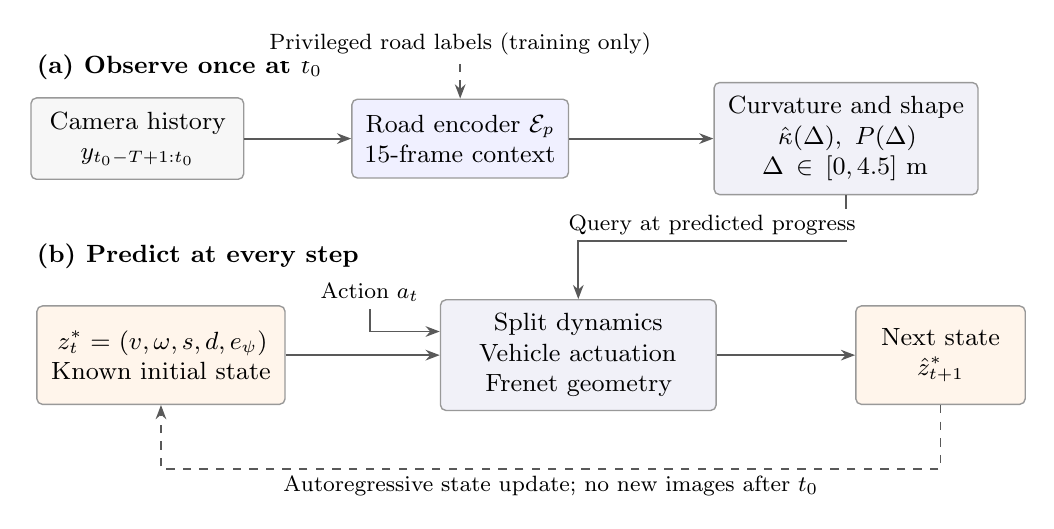
\begin{tikzpicture}[x=1cm,y=1cm,font=\fontsize{9}{11}\selectfont,
 box/.style={draw=black!40,rounded corners=2pt,line width=.5pt,align=center,inner sep=5pt},
 ar/.style={-{Stealth[length=1.8mm]},line width=.7pt,draw=black!65},
 lab/.style={font=\fontsize{8}{10}\selectfont,fill=white,inner sep=2pt}]
\node[anchor=west,font=\bfseries\fontsize{9}{11}\selectfont] at (0,4.05) {(a) Observe once at $t_0$};
\node[box,fill=black!3,text width=2.35cm,minimum height=1cm] (cam) at (1.4,3.15)
 {Camera history\\$y_{t_0-T+1:t_0}$};
\node[box,fill=blue!6,text width=2.4cm,minimum height=1cm] (enc) at (5.5,3.15)
 {Road encoder $\mathcal E_p$\\15-frame context};
\node[box,fill=frenetink!7,text width=3cm,minimum height=1cm] (preview) at (10.4,3.15)
 {Curvature and shape\\$\hat\kappa(\Delta),\ P(\Delta)$\\$\Delta\in[0,4.5]$ m};
\draw[ar] (cam) -- (enc);
\draw[ar] (enc) -- (preview);
\node[lab,anchor=south] at (5.5,4.13) {Privileged road labels (training only)};
\draw[ar,dashed] (5.5,4.1) -- (enc.north);
\node[anchor=west,font=\bfseries\fontsize{9}{11}\selectfont] at (0,1.65) {(b) Predict at every step};
\node[box,fill=orange!8,text width=2.8cm,minimum height=1.25cm] (state) at (1.7,.4)
 {$z_t^*=(v,\omega,s,d,e_\psi)$\\Known initial state};
\node[box,fill=frenetink!7,text width=3.15cm,minimum height=1.25cm] (dyn) at (7.0,.4)
 {Split dynamics\\Vehicle actuation\\Frenet geometry};
\node[box,fill=orange!8,text width=1.8cm,minimum height=1.25cm] (next) at (11.6,.4)
 {Next state\\$\hat z^*_{t+1}$};
\draw[ar] (state) -- (dyn);
\draw[ar] (dyn) -- (next);
\draw[ar] (preview.south) -- (10.4,1.85) -- node[lab,above] {Query at predicted progress} (7,1.85) -- (dyn.north);
\node[lab] at (4.35,1.2) {Action $a_t$};
\draw[ar] (4.35,.98) |- ([yshift=3mm]dyn.west);
\draw[ar,dashed] (next.south) -- (11.6,-1.05) -- node[lab,below] {Autoregressive state update; no new images after $t_0$} (1.7,-1.05) -- (state.south);
\end{tikzpicture}
\caption{Implemented prediction pathways. The camera supplies curvature and shape once per rollout; annotated state initializes the dynamics. Recorded actions drive subsequent updates. The original and guarded variants query the curvature head; the consistent variant derives curvature and parameter speed from the shape curve. Position is decoded using that predicted curve, without surveyed-map queries during rollout. Initial road-relative state remains privileged.}
\label{fig:arch}
\end{figure}
\subsection{Road-preview encoder}\label{sec:repr_learning}\label{sec:encoding}
A convolutional encoder receives the red channel of 15 consecutive $64\times64$
frames, stacked as channels and scaled to $[0,1]$. Four convolutions have
32, 64, 128, and 256 channels, kernel size 4, stride 2, and padding 1. The
flattened output feeds a 256-unit fully connected layer. This feature
vector feeds linear heads for ten curvature samples and twenty centerline
coordinates. The longitudinal shape output is a residual relative to nominal
offsets; the lateral output is direct. Joint supervised squared error is
normalized by training-set output standard deviations, floored at 0.05 in the
corresponding units. The controlled experiment does not use an image autoencoder,
VQ codebook, Transformer, or joint perception/dynamics fine-tuning.

The original encoder uses ReLU and outputs directly in physical units.
An exploratory repair uses LeakyReLU with slope 0.01 and
$\hat y=\mu_{\rm train}+\sigma_{\rm train}r_\theta$, retaining width, depth,
loss, and training budget. All six encoders are retrained under this rule.
Changing activation and output parameterization together prevents isolating
their individual causal contributions.

\subsection{Road-relative dynamics}\label{sec:prediction}
For an arc-length centerline within its valid coordinate chart, slip-free
kinematics gives
\begin{align}
 \dot s&=\frac{v\cos\psi}{1-d\kappa},\label{eq:frenet_s}\\
 \dot d&=v\sin\psi,\label{eq:frenet_d}\\
 \dot\psi&=\omega-\kappa\dot s.\label{eq:frenet_psi}
\end{align}
The independently predicted curve and legacy map labels only approximate
these arc-length identities; the original and guarded models are structured
predictors rather than exact physical coordinate transformations. The
consistent variants below explicitly address this distinction.
The implementation adds learned lateral and heading residuals and per-step
increments in speed and yaw rate. Three multilayer perceptrons, each with two 64-unit ReLU hidden layers, consume
normalized $d,\psi,v,\omega,\kappa$ and actions. These actuation increments are
not recovered physical bicycle parameters. The original variant uses Euler
updates, interpolated curvature from the visual head, and a separate predicted
centerline for reconstruction.

A cubic Hermite interpolant $P(s)$ uses centered interior tangents, an initial
road-$x$ tangent, and a final chord tangent. With tangent heading $\theta(s)$,
the vehicle position is $P(s)+d[-\sin\theta(s),\cos\theta(s)]^{\mathsf T}$ and
heading is $\theta(s)+\psi$. An ego transform removes initial translation and
rotation. Outside the 4.5 m preview, the position readout extends its endpoint
tangent while the independent curvature head holds its last value. These two
extensions are not generally geometrically consistent.

\paragraph{Numerical safeguards}
The guarded variant uses $\max(0.2,1-d\kappa)$, wraps heading, and bounds learned
increments with hyperbolic tangents. Speed and yaw-rate bounds are training-only
99.5th percentiles of absolute one-frame changes, floored at 0.01 in their
respective units. Lateral and heading residual limits are 0.1 m and 0.1 rad
per step. Positive denominator protection extends the numerical update outside
its valid chart; it does not make such states physically valid. We record states
with $1-d\kappa\leq0$. Finite increments imply neither bounded states nor
bounded prediction errors.

\paragraph{Geometric consistency}
Nominal arc-length knots do not guarantee a unit-speed predicted interpolant.
Let $q$ be its actual parameter, $g=\|P'(q)\|$, and
$\kappa_P=\det(P'(q),P''(q))/g^3$. Consistent dynamics requires
\begin{equation}
 \dot q=\frac{v\cos\psi}{g(1-d\kappa_P)},\qquad
 \dot\psi=\omega-\kappa_Pg\dot q.\label{eq:consistent_geometry}
\end{equation}
We evaluate this correction with Euler and explicit midpoint integration, using
the same curve in dynamics and readout. The independent curvature head is
ignored, $g$ is floored at 0.1, and the other safeguards are retained.
Tangent extension uses $g=1$ and $\kappa_P=0$ outside the preview.
Synthetic checks assess readout equivalence, finite-difference derivatives,
and the coordinate-to-Cartesian velocity identity. Consistency does not imply
that the predicted curve matches the real road.

\subsection{Controls and training}\label{sec:baselines}
A calibrated kinematic control learns seven global coefficients for throttle
gain, drag, effective length, steering gain and bias, drive bias, and yaw-response
lag. It receives initial speed, yaw rate, and future actions, without road inputs.
Two Cartesian residual controls have the same architecture; one receives the
initial road state and frozen visual preview, and the other zeros these inputs.
Their residual network has two 96-unit ReLU hidden layers and five outputs.
Its inputs are scaled planar position, sine/cosine of heading, normalized speed
and yaw rate, two actions, and 32 normalized road-context quantities. Both learn
residuals to analytic planar kinematics. These implementations are
not claimed reproductions of DVBF, GOKU-net, or Vid2Param. Constant speed and yaw
rate provide an additional action-independent diagnostic.

Perception training uses 25 epochs, Adam with initial learning rate $10^{-3}$,
cosine decay, batch size 64, and frame stride 2. The checkpoint minimizes
validation normalized supervision loss. Dynamics use 40 epochs, 32-step windows,
batch size 128, stride 4, and a common physical-output loss. Initial learning
rates are $10^{-3}$ for neural dynamics and $10^{-2}$ for calibrated kinematics,
with cosine decay. Gradient norms are clipped at 1 for dynamics and 5 for
perception. Dynamics checkpoints minimize validation 100-step endpoint error.
All seeds (0, 1, 2) are retained.

The loss averages squared errors in ego-frame $x,y$, wrapped heading, speed,
and yaw rate, scaled by 0.5 m, 0.5 m, 0.5 rad, and training standard deviations
of speed and yaw rate (floored at 0.01). Evaluation errors do not choose
checkpoints within these runs; choices between modeling rounds are exploratory
because earlier results had already been inspected.

\section{Experimental Evaluation}\label{sec:experiments}\label{sec:setup}
\subsection{Data and source-separated protocol}
The physical archive contains two recordings with 5801 and 13597 frames at
approximately 22 Hz, including images, steering/throttle, logged planar pose,
speed, and a track map. Preprocessing yields 18 and 53 usable segments.
These segments share acquisition conditions and layout; they are not independent
sessions. Yaw rate uses at most five past yaw differences.

Direction A evaluates the first source, with 41 training, 11 validation, and one
purged segment from the second source. Direction B evaluates the second source,
with 13 training, 4 validation, and one purged segment from the first.
Validation is the final 20\% of ordered development-source segments; at least
115 original frames separate training and validation. Evaluation uses 844 and
1653 overlapping windows with stride 4 and horizon 100 (approximately 4.55 s).

Learned parameters and normalization statistics use training data only. Each
round freezes its protocol, implementation hashes, and required input checkpoints
before fitting; evaluation waits for all prescribed runs. Audits check data and
checkpoint hashes, validation selection, window identity, recomputed metrics,
and zero initial position error.

Both recordings were previously used in development. Retained track preprocessing
also includes orientation chosen using the first recording and historically
explored grid settings. Separation therefore concerns present fitting and
checkpoint selection, not a prospectively untouched complete pipeline.
No unseen-track or new-recording generalization claim follows.


\paragraph{Operating regimes and identifiability}
Across retained frames, median speeds are 0.434 and 0.774 m/s in the two records.
The first has constant throttle 0.566667, whereas the second ranges from
0.633333 to 0.766667. Source separation therefore also probes changes in operating
regime. In a model $\dot v=k_a u-k_dv+b$, constant $u=c$ identifies the combination
$k_ac+b$, not $k_a$ and $b$ separately: replacing them by $k_a+\Delta$ and
$b-c\Delta$ leaves the update unchanged. We do not interpret fitted coefficients
as uniquely recovered physical parameters. This limitation does not by itself
explain all prediction errors.

\subsection{Metrics}

Endpoint error is
\begin{equation}
 E_{xy}(k)=\frac1N\sum_{i=1}^{N}\|\hat p_{i,k}-p_{i,k}\|_2.\label{eq:metric_exy}
\end{equation}
We report steps 25, 50, and 100, plus mean error over steps 1--100 (ADE), in meters.
Mean $\pm$ standard deviation summarizes three training seeds, not uncertainty
across independent recording sessions. Overlapping windows are not independent
trials for significance testing. The primary metric is 100-step endpoint error.

\subsection{Earlier experiments}
Conference CartPole, Lunar Lander, and DonkeyCar-simulator results are retained
with attribution~\cite{piwm_conf}. Their supervision and architectures differ
from the current road encoder. CarRacing was a development environment, but this
article has no completed quantitative CarRacing validation of the road-context
model. Earlier five-fold physical-car results are preserved in
Appendix~\ref{sec:historical}, under their original information and selection
conditions; they cannot be pooled with the new source-separated estimates.

\section{Results}\label{sec:results}
\subsection{Initial controlled comparison}\label{sec:donkeyreal_results}
Table~\ref{tab:controlled} shows lower mean Frenet endpoint error than the
road-conditioned Cartesian residual control in both directions, but calibrated
kinematics is better in both. These findings concern the specified implementations
and budgets, rather than all possible models in either coordinate system.
\begin{table}[t]
\centering
\caption{Initial retrospective comparison. Errors in m; mean $\pm$ sample SD over three seeds. A and B evaluate the first and second original recordings.}
\label{tab:controlled}
\footnotesize
\setlength{\tabcolsep}{3pt}
\begin{tabular}{lrrrr}
\toprule
Model & A: $E_{100}$ & A: ADE & B: $E_{100}$ & B: ADE \\
\midrule
Calibrated kinematics & $0.936 \pm 0.005$ & $0.455 \pm 0.002$ & $1.158 \pm 0.006$ & $0.595 \pm 0.002$ \\
Cartesian, no road & $1.230 \pm 0.128$ & $0.654 \pm 0.082$ & $1.466 \pm 0.156$ & $0.720 \pm 0.049$ \\
Cartesian, road & $1.344 \pm 0.223$ & $0.679 \pm 0.063$ & $1.653 \pm 0.035$ & $0.692 \pm 0.014$ \\
Frenet & $1.086 \pm 0.150$ & $0.608 \pm 0.112$ & $1.463 \pm 0.037$ & $0.688 \pm 0.022$ \\
\bottomrule
\end{tabular}
\end{table}

Replacing both curvature and shape by a straight road raises Frenet endpoint
error to $2.129\pm0.546$ and $2.415\pm0.071$ m. Setting curvature alone to zero
while keeping shape gives $0.994\pm0.126$ and $1.517\pm0.069$ m. The joint
intervention therefore does not isolate curvature-dependent dynamics.
Inference-time interventions also introduce distribution shift; separately
trained ablations provide a complementary comparison.

\subsection{Numerical stability and retrained ablations}
Two original Frenet runs deteriorate after their validation-optimal epochs:
final validation errors reach 99.875 and 21.681 m, with maximum pre-clipping
gradient norms above $10^{12}$ and $10^{13}$. Selected checkpoints reproduce the
initial comparison exactly in the diagnostic rerun. Guarded updates avoid these
extreme failures in the same runs, but can still leave the valid Frenet chart.

Table~\ref{tab:guards} reports models refit with fixed perception. Shape-only
sets curvature to zero throughout fitting and prediction. No-road additionally
replaces shape by a straight line and zeros initial road-relative displacement
and heading; it does not isolate shape alone. The oracle receives true curvature
and shape during fitting and evaluation; it is not a theoretical upper bound.
\begin{table}[t]
\centering
\caption{Exploratory numerical safeguards and retrained ablations using the original frozen encoders.}
\label{tab:guards}
\footnotesize
\setlength{\tabcolsep}{3pt}
\begin{tabular}{lrrrr}
\toprule
Model & A: $E_{100}$ & A: ADE & B: $E_{100}$ & B: ADE \\
\midrule
Guarded, full & $1.022 \pm 0.154$ & $0.473 \pm 0.062$ & $1.432 \pm 0.019$ & $0.672 \pm 0.025$ \\
Guarded, shape only & $0.846 \pm 0.048$ & $0.400 \pm 0.046$ & $1.471 \pm 0.062$ & $0.688 \pm 0.025$ \\
Guarded, no road & $1.029 \pm 0.078$ & $0.492 \pm 0.012$ & $1.579 \pm 0.161$ & $0.675 \pm 0.058$ \\
Guarded, oracle & $0.933 \pm 0.068$ & $0.430 \pm 0.035$ & $1.285 \pm 0.039$ & $0.618 \pm 0.020$ \\
\bottomrule
\end{tabular}
\end{table}

Shape-only improves on the full model in A but worsens it in B. Neither the
safeguards nor the oracle establishes a consistent advantage over calibrated
kinematics, so the remaining gap cannot be attributed solely to perception.

\subsection{Geometric consistency and integration}
A validation-only audit finds that predicted curves are not generally unit-speed
in their nominal parameter. For one encoder, 80.1\% of sampled locations have
$|g-1|>0.2$. Independent and shape-derived curvatures also disagree. Even the
coarse oracle interpolant is not exactly unit-speed. Synthetic checks verify
the coordinate velocity identity in Eq.~\eqref{eq:consistent_geometry}.
On a synthetic circle, zero-residual 100-step endpoint error falls from
0.001293 m with Euler to 0.000119 m with midpoint integration. This checks the
numerical implementation, not accuracy on recorded driving.

Table~\ref{tab:geometry} evaluates consistent dynamics with the original encoders.
The body midpoint control uses the same network structure and integrator, but
clears road inputs. Geometry helps relative to this control in B; A has the
opposite ordering. Calibrated kinematics still gives lower mean endpoint error
in both directions.
\begin{table}[t]
\centering
\caption{Exploratory geometry and integration controls with the original encoders.}
\label{tab:geometry}
\footnotesize
\setlength{\tabcolsep}{3pt}
\begin{tabular}{lrrrr}
\toprule
Model & A: $E_{100}$ & A: ADE & B: $E_{100}$ & B: ADE \\
\midrule
Consistent, Euler & $1.141 \pm 0.051$ & $0.537 \pm 0.035$ & $1.314 \pm 0.034$ & $0.611 \pm 0.029$ \\
Consistent, midpoint & $1.267 \pm 0.361$ & $0.571 \pm 0.138$ & $1.325 \pm 0.042$ & $0.609 \pm 0.035$ \\
Body, midpoint & $1.009 \pm 0.056$ & $0.486 \pm 0.078$ & $1.793 \pm 0.221$ & $0.775 \pm 0.069$ \\
\bottomrule
\end{tabular}
\end{table}

\subsection{Visual conditioning and matched dynamics}
Training and validation logs identify one encoder with nearly constant outputs.
Its best normalized validation loss is 0.8384, versus 0.1220 and 0.1280 for the
other seeds in that direction. This diagnoses representation collapse, not its
precise optimization mechanism. Uniform conditioning repair improves validation
loss in five of six runs; one changes from 0.1220 to 0.1371. The collapsed run
improves to 0.2953 with nonconstant outputs. Validation improvements alone do
not demonstrate improved trajectory generalization.
\begin{table}[t]
\centering
\caption{Matched dynamics with six uniformly retrained conditioned encoders. All dynamics are refit from scratch; all variants and seeds are retained.}
\label{tab:conditioned}
\footnotesize
\setlength{\tabcolsep}{3pt}
\begin{tabular}{lrrrr}
\toprule
Model & A: $E_{100}$ & A: ADE & B: $E_{100}$ & B: ADE \\
\midrule
Guarded, full & $0.951 \pm 0.089$ & $0.435 \pm 0.035$ & $1.387 \pm 0.038$ & $0.672 \pm 0.010$ \\
Guarded, shape only & $0.870 \pm 0.108$ & $0.375 \pm 0.058$ & $1.394 \pm 0.026$ & $0.663 \pm 0.022$ \\
Consistent, midpoint & $1.020 \pm 0.088$ & $0.469 \pm 0.046$ & $1.300 \pm 0.068$ & $0.616 \pm 0.044$ \\
Cartesian, road & $1.402 \pm 0.113$ & $0.667 \pm 0.041$ & $1.584 \pm 0.040$ & $0.680 \pm 0.029$ \\
\bottomrule
\end{tabular}
\end{table}
Table~\ref{tab:conditioned} uses the same previously examined sources. The
consistent model ignores the independent curvature head, while shape-only clears
that head during dynamics. Neither ablation isolates curvature supervision of
the jointly trained encoder. The kinematic and no-road Cartesian references in
Table~\ref{tab:controlled} are unaffected by encoder changes.

\begin{figure}[t]
\centering
\includegraphics[width=\linewidth]{fig_conditioned_comparison.pdf}
\caption{Complete conditioned-dynamics comparison and fixed controls. Lines are
means over three training seeds; shading is sample standard deviation across
seeds, not a confidence interval over recording sessions. All curves use the
same source-specific windows, privileged initialization, and recorded actions.
Both sources had been inspected in earlier development.}
\label{fig:conditioned_comparison}
\end{figure}

\subsection{Purged temporal prediction within both sources}\label{sec:temporal}
To distinguish source/regime transfer from forecasting within recorded operating
conditions, we add an exploratory chronological split separately within each
source. The first approximately 60\% of ordered segments train the models,
the next 20\% select checkpoints, and the last 20\% evaluate them. Boundary
segments are purged to leave at least 115 original frames between adjacent
partitions. This produces 9+30 training segments, 3+10 validation segments,
4+11 evaluation segments, and 2+2 purged segments.
All encoders and six dynamics variants are trained from scratch using the same
25/40-epoch budgets. The guarded full model and pooled-window endpoint metric
are fixed before fitting; no family is selected retrospectively as the winner.

This experiment was designed after inspecting the earlier studies and the
recorded operating ranges. It does not provide fresh independent confirmation,
and it does not replace the source-held-out stress tests. The narrower question
is prediction on later portions of the same sources, with both sources represented
during training. Training throttle nevertheless contains only 0.566667 and
0.633333, whereas the second full record reaches 0.766667. This split is not
asserted to be identically distributed or to cover every later operating condition. Table~\ref{tab:temporal} reports the pooled primary
metric and both source-specific endpoint errors.
\begin{table}[t]
\centering
\caption{Exploratory chronological holdout with both sources represented during training; later operating shifts may remain. Pooled-window E100 is primary; the last two columns expose the original sources separately. Errors in m, mean and sample SD over three seeds.}
\label{tab:temporal}
\footnotesize
\setlength{\tabcolsep}{3pt}
\begin{tabular}{lrrrr}
\toprule
Model & Pooled $E_{100}$ & Pooled ADE & Rec. 1 $E_{100}$ & Rec. 2 $E_{100}$ \\
\midrule
Calibrated kinematics & $0.898 \pm 0.006$ & $0.437 \pm 0.004$ & $0.858 \pm 0.006$ & $0.913 \pm 0.005$ \\
Cartesian, no road & $0.930 \pm 0.335$ & $0.367 \pm 0.081$ & $0.675 \pm 0.355$ & $1.029 \pm 0.329$ \\
Cartesian, road & $1.095 \pm 0.212$ & $0.424 \pm 0.090$ & $0.793 \pm 0.310$ & $1.211 \pm 0.175$ \\
Guarded, full & $0.343 \pm 0.010$ & $0.197 \pm 0.005$ & $0.208 \pm 0.028$ & $0.395 \pm 0.004$ \\
Guarded, shape only & $0.412 \pm 0.018$ & $0.246 \pm 0.015$ & $0.260 \pm 0.019$ & $0.471 \pm 0.026$ \\
Consistent, midpoint & $0.372 \pm 0.028$ & $0.208 \pm 0.012$ & $0.301 \pm 0.042$ & $0.399 \pm 0.023$ \\
\bottomrule
\end{tabular}
\end{table}
The prespecified guarded full model gives a pooled endpoint error of 0.343 m, compared with 0.898 m for calibrated kinematics and 1.095 m for the road-conditioned Cartesian control. These values must be interpreted together with the per-source results and the cross-source stress tests, not as evidence for unseen-track generalization.

\subsection{A single unit-speed road representation}\label{sec:coupled}
The preceding consistency audit motivates an exploratory encoder whose curvature
and position describe one curve by construction. Ten predicted curvature knots
replace the independent curvature and shape heads. For the nine intervals of
length $\ell=0.5$ m, let $\bar\kappa_j=(\hat\kappa_j+\hat\kappa_{j+1})/2$ and
$\theta_j=\sum_{i<j}\bar\kappa_i\ell$. At distance $u\in[0,\ell]$ in interval $j$,
\begin{align}
 C(q_j+u)&=C(q_j)+u\,\operatorname{sinc}(\bar\kappa_j u/2)
 \begin{bmatrix}\cos(\theta_j+\bar\kappa_j u/2)\\
 \sin(\theta_j+\bar\kappa_j u/2)\end{bmatrix},\\
 \theta(q_j+u)&=\theta_j+\bar\kappa_j u,
\end{align}
where $\operatorname{sinc}(x)=\sin(x)/x$, extended continuously at zero.
Position and tangent are continuous; curvature can jump at interval boundaries.
The curve has unit parameter speed, and the same interval curvature drives
midpoint Frenet updates and position readout. Outside the preview, tangent
extension has zero curvature. This is a consistent implementation of standard
curve geometry, not a new Frenet identity or a stability guarantee.

The encoder retains the conditioned CNN backbone and is jointly supervised by
legacy curvature and shape targets; shape gradients propagate through the arc
integral. All three seeds are refit for 25 epochs. Four dynamics variants are
refit for 40 epochs on exactly the temporal split in Section~\ref{sec:temporal}.
The full coupled model and pooled $E_{100}$ are fixed before fitting. The
independent-encoder control uses the preceding frozen CNN's curvature output
with the same arc decoder and dynamics. The shape-only variant removes
curvature from the dynamics but retains the curved readout; it does not remove
all curvature information. Cartesian dynamics receives the same coupled preview.
\begin{table}[t]
\centering
\caption{Exploratory coupled representation on the unchanged chronological split. Mean and sample SD over all three seeds; all variants retained.}
\label{tab:coupled}
\footnotesize
\setlength{\tabcolsep}{3pt}
\begin{tabular}{lrrrr}
\toprule
Model & Pooled $E_{100}$ & Pooled ADE & Rec. 1 $E_{100}$ & Rec. 2 $E_{100}$ \\
\midrule
Coupled arc, full & $0.400 \pm 0.005$ & $0.217 \pm 0.001$ & $0.260 \pm 0.008$ & $0.454 \pm 0.005$ \\
Coupled arc, shape only & $0.454 \pm 0.042$ & $0.259 \pm 0.026$ & $0.260 \pm 0.040$ & $0.529 \pm 0.053$ \\
Arc, independent encoder & $0.468 \pm 0.022$ & $0.235 \pm 0.009$ & $0.314 \pm 0.021$ & $0.528 \pm 0.023$ \\
Cartesian, coupled road & $1.080 \pm 0.021$ & $0.414 \pm 0.022$ & $0.722 \pm 0.051$ & $1.218 \pm 0.035$ \\
\bottomrule
\end{tabular}
\end{table}
The full coupled model has pooled endpoint error 0.400 m, compared with 0.468 m for the independent-encoder arc control and 1.080 m for Cartesian dynamics using the coupled preview. The unchanged calibrated-kinematic reference is 0.898 m. These comparisons jointly expose coupling, geometry, and model-family effects.

\begin{figure}[t]
\centering
\includegraphics[width=\linewidth]{fig_temporal_comparison.pdf}
\caption{Chronological-holdout errors for every prescribed variant. The panels
separate the independent-head and coupled-road suites; calibrated kinematics
is repeated as a common reference. Means and shading summarize three seeds
(sample standard deviation), not independent recording uncertainty.}
\label{fig:temporal_comparison}
\end{figure}

\subsection{Compatibility of the geometric supervision}
The persisted centerline is smoothed after resampling and is not reparameterized
by arc length afterward. Its nominal grid length is 10.450 m,
whereas the smoothed polygon length is 9.743 m. At the native 0.05 m grid,
the median absolute deviation of parameter speed from one is 0.0512.
Stored curvature is additionally smoothed. Thus these direct map-derived labels
are not exact, mutually consistent geometric ground truth.

On the temporal validation windows, integrating the stored curvature with the
piecewise-arc decoder differs from the stored shape by 0.207 m
coordinate RMSE. This difference combines map parameterization, separate
curvature smoothing, and coarse interval approximation; it does not isolate one
cause. Joint supervision of an exact unit-speed representation therefore
introduces target mismatch. No test-window information is used in this audit,
and the existing targets and complete experimental results are retained.
This limits conclusions about the best attainable accuracy of geometrically
consistent learning from corrected labels.
For the fixed guarded full model, seed-averaged endpoint error improves on calibrated kinematics and both Cartesian controls in all 14 eligible temporal test segments. Only 14 of the 15 assigned segments are long enough for the prescribed 15-frame context and 100-step horizon, yielding 527 windows. Full dynamics improves on shape-only in 10 of those segments. This is descriptive paired evidence: overlapping windows and segments from two recordings do not provide 14 independent acquisition sessions.
The maximum fraction of monitored full-step states with an invalid Frenet denominator in the guarded full model is 0.0569\%. Finite rollouts therefore do not establish chart validity. Midpoint internal stages are not included in this monitoring.
\begin{figure}[t]
\centering
\includegraphics[width=\linewidth]{fig_conference_environments.pdf}
\caption{Original conference environments: CartPole, Lunar Lander and the
DonkeyCar simulator. Frames are extracted from the ground-truth rows of the
conference qualitative figures~\cite{piwm_conf}; the simulated driving scene
is distinct from the physical platform evaluated in the present study.}
\label{fig:conf_environments}
\end{figure}
\subsection{Retained Conference Benchmark Results}\label{sec:conf_results}

We restore the original conference results~\cite{piwm_conf} in
Figures~\ref{fig:conf_cartpole}--\ref{fig:conf_rollouts}. These are inherited
experiments, not additional runs of PIWM-Frenet. They compare intrinsic and
extrinsic encoders with continuous or discrete latents over 30 prediction steps
and supervision-noise levels $\delta\in\{0,5\%,10\%\}$. The conference protocol
uses five-fold cross-validation. State RMSE in these benchmarks is distinct from
the meter-valued position error of the physical-car evaluation.

\paragraph{Prediction and architectural choice}
Figures~\ref{fig:conf_cartpole}, \ref{fig:conf_lunar} and
\ref{fig:conf_donkey} retain all six panels for each environment. Extrinsic
PIWM with discrete latents gives the lowest long-horizon error among the
extrinsic variants shown. The intrinsic setting has a different ranking:
continuous PIWM generally outperforms the discrete variant. Thus the conference
results support choosing the latent parameterization together with the encoder
architecture, rather than a universal advantage for quantization. The driving
encoder comparison in Table~\ref{tab:kappa_source} revisits this choice for the
new road-perception task.

\begin{figure}[p]
\centering
\includegraphics[width=\linewidth]{fig_conference_cartpole.pdf}
\caption{Conference CartPole results~\cite{piwm_conf}. State RMSE over 30 steps
for (a) extrinsic and (b) intrinsic methods, under three supervision-noise
levels. Curves and shaded regions are the original embedded plot images;
labels and layout have been reset. Panel-specific vertical limits are retained.
The archived figure does not specify the statistical meaning of its shading.}
\label{fig:conf_cartpole}
\end{figure}

\begin{figure}[p]
\centering
\includegraphics[width=\linewidth]{fig_conference_lunar.pdf}
\caption{Conference Lunar Lander results~\cite{piwm_conf}. The layout and
method groups follow Figure~\ref{fig:conf_cartpole}. Original curves and shaded
regions are preserved; all panels retain the source RMSE range $[0,2]$.}
\label{fig:conf_lunar}
\end{figure}

\begin{figure}[p]
\centering
\includegraphics[width=\linewidth]{fig_conference_donkey.pdf}
\caption{Conference DonkeyCar-simulator results~\cite{piwm_conf}. The layout
follows Figure~\ref{fig:conf_cartpole}. Original curves and shaded regions are
preserved, including the source vertical limit of 2; curves beyond that limit
are clipped as in the original. These are 30-step state-RMSE results and must
not be read as the 100-step position errors of the physical car.}
\label{fig:conf_donkey}
\end{figure}

\paragraph{Parameter estimates and visual rollouts}
Figure~\ref{fig:conf_parameters} restores the parameter comparison for CartPole
and Lunar Lander. The reference lines make both agreement and departures from
the known parameters visible as supervision noise changes. We omit the original
DonkeyCar wheelbase panel from this recovery comparison because it has no
known-parameter reference. Figure~\ref{fig:conf_rollouts} retains all five
comparison rows from the original visual rollout example, with three
display columns selected for legibility. These examples illustrate visual
behavior and do not replace the quantitative comparisons above. The original controller diagnostic is also
retained in Appendix~\ref{sec:conf_control}.

\begin{figure}[p]
\centering
\includegraphics[width=\linewidth]{fig_conference_parameters.pdf}
\caption{Conference parameter estimates for the two controlled
benchmarks~\cite{piwm_conf}. Each panel retains the original colored intervals,
center marks and yellow ground-truth reference. Rows correspond to
$\delta=0,5\%,10\%$, from top to bottom. Parameter names and scales follow the
source figure; the source does not specify the interval statistic.}
\label{fig:conf_parameters}
\end{figure}

\begin{figure}[p]
\centering
\includegraphics[width=\linewidth]{fig_conference_rollouts.pdf}
\caption{Conference visual rollouts at $\delta=5\%$~\cite{piwm_conf}.
Ground truth and the four original model rows are shown at $k=5,15,30$ for the
DonkeyCar simulator and Lunar Lander. Frames are extracted without retouching;
the intermediate display columns and the slide footer have been omitted.}
\label{fig:conf_rollouts}
\end{figure}
\FloatBarrier


\section{Discussion}\label{sec:discussion}
The studies distinguish physical meaning, numerical behavior, and predictive
accuracy. The first two do not imply the third. Named variables expose coordinate
failures and inconsistent geometric representations, as the audits demonstrate.
Accuracy benefits depend on the recording, split, baseline, and implementation.
The chronological-holdout gains are substantial and reproducible from saved
weights, but the protocol was designed during development on reused sources.
They support within-source prediction under the stated information conditions,
while the source-separated results expose limited transfer.

Road geometry alone does not alter action-conditioned planar kinematics. As
context for learned actuation, it may encode correlations with driving conditions
or the behavior generating the data. These experiments do not identify such
correlations as causal effects. Re-indexing a fixed preview removes one learned
recurrent update but still propagates errors in progress and geometry.

The principal limitation is two reused recordings on one track. Seeds assess
optimization variability, not variation across independent tracks, vehicles,
or acquisition sessions. Successive repairs were informed by previous analysis;
their evaluation is exploratory even with validation-only checkpoint selection.
Fresh acquisition is needed for prospective confirmation of a selected method.
Other limitations are privileged initialization, map-derived encoder labels, recorded
future actions, finite preview, and absence of closed-loop assessment. Numerical
guards can remain finite outside the valid coordinate chart. No safety or
general bounded-error guarantee follows.

The direct road encoder differs from the conference autoencoding pipeline, whose
weak-supervision results do not establish weakly supervised road perception.
Historical reduced baselines also cannot establish superiority over the full
published methods. A deployment accuracy claim requires benefits over calibrated
dynamics across independent conditions and evaluation with an initial-state
estimator. Favorable subsets of these development experiments cannot satisfy
those requirements.

\section{Conclusion}\label{sec:conclusion}
We developed and audited a camera-derived road-context extension of PIWM for
offline action-conditioned prediction. Explicit geometry makes coordinate
assumptions and failures inspectable. Controlled studies distinguish input
information, reconstruction, numerical safeguards, and dynamics training.
The original Frenet predictor does not beat calibrated kinematics in the two
source-held-out directions. The guarded model substantially improves chronological prediction
over matched controls, with improvements in both recordings and across all
eligible test segments against the three principal baselines. This contrast
with source-transfer performance identifies a useful but limited operating
regime for the representation; geometric consistency alone is insufficient
to establish predictive superiority.
The evidence supports a limited empirical account of the representation, not
resolved partial observability, camera-only deployment, or guaranteed stability.

\section*{Declaration of Competing Interest}
%% ==============================================================

%% TODO(authors): confirm before submission and adjust if any author has a
%% competing interest to declare.
[AUTHOR CONFIRMATION REQUIRED: competing-interest declaration.]

%% ==============================================================
\section*{CRediT Authorship Contribution Statement}
%% ==============================================================

%% TODO(authors): fill in per-author CRediT roles once the author list is fixed.
%% Example: \textbf{Jane Doe}: Conceptualization, Methodology, Software,
%% Investigation, Writing --- original draft.
[CRediT ROLES --- TO BE COMPLETED BEFORE SUBMISSION.]

%% ==============================================================
\section*{Data Availability}
%% ==============================================================

%% TODO(authors): replace with the archived DOI / repository URL before
%% submission, or state the applicable restriction.
[AUTHOR CONFIRMATION REQUIRED: data/code release location, permissions, and access restrictions.]

%% ==============================================================
\section*{Acknowledgements}
%% ==============================================================

The authors thank Liam (Cade) McGlothlin and Vedansh Maheshwari for their help in
exploring interpretable world models.
This material is based upon work supported by the U.S.\ National Science Foundation
under Grant Numbers CNS~2513076 and CCF~2403616.
Any opinions, findings, and conclusions expressed in this material are those of the
authors and do not necessarily reflect the views of the NSF.


%% ==============================================================
\section*{Declaration of Generative AI Use}
[AUTHOR REVIEW REQUIRED BEFORE SUBMISSION.] GPT-6 (Codex) assisted with code
inspection, experimental implementation, analysis, and manuscript revision.
The final disclosure requires author verification of its scope and compliance
with the journal policy. This draft does not assert that the authors have
already verified or approved all assisted outputs.

\appendix
\section{Historical Physical-Car Development Results}\label{sec:historical}
These tables and figures preserve earlier five-fold development results.
The 71 segments come from the same two recordings. Displayed evaluation windows
also selected dynamics checkpoints, so these estimates are optimistic as measures
of generalization. The original Vid2Param visual encoder was shared across folds;
DVBF and GOKU-net were reduced to dynamics-only variants. Budgets and information
pathways differed. These are descriptive results under the original protocol,
not a clean ranking of published methods.

The 0.463 m result uses surveyed-map position reconstruction and privileged
initialization. The 0.516 m row uses perceived-shape readout with the original
selection and initialization conditions. Differences from the source-separated
study also involve splits, losses, horizons, and readout implementation; they
are not a controlled estimate of one isolated source of optimism.
\begin{table}[t]
\centering
\caption{Historical five-fold development errors (m). Displayed windows also selected checkpoints. Frenet uses map-assisted readout except in the map-free row; all rows use privileged initialization. Baseline names refer to local reduced implementations. These are not independent test estimates.}
\label{tab:donkey_main}
\footnotesize
\setlength{\tabcolsep}{3.4pt}
\begin{tabular}{lrrr}
\toprule
Model & $E_{xy}(25)$ & $E_{xy}(50)$ & $E_{xy}(100)$ \\
\midrule
Vid2Param~\cite{asenov2019vid2param}   & $\mathbf{0.036 \pm 0.008}$ & $\mathbf{0.107 \pm 0.008}$ & $0.703 \pm 0.142$ \\
GOKU-net~\cite{linial_generative_2021}  & $0.046 \pm 0.012$ & $0.131 \pm 0.013$ & $0.725 \pm 0.107$ \\
DVBF~\cite{karl2016deep}               & $0.061 \pm 0.011$ & $0.173 \pm 0.031$ & $0.837 \pm 0.131$ \\
SINDYc~\cite{BRUNTON2016710}           & \multicolumn{3}{c}{diverges in all $2483$ windows of all five folds} \\
\midrule
\textbf{PIWM-Frenet (ours, perceived $\kappa$)} & $0.141 \pm 0.009$ & $0.245 \pm 0.021$ & $\mathbf{0.463 \pm 0.045}$ \\
\emph{PIWM-Frenet (map-free)} & \emph{$0.146 \pm 0.012$} & \emph{$0.258 \pm 0.023$} & \emph{$0.516 \pm 0.056$} \\
\bottomrule
\end{tabular}
\end{table}
\begin{table}[t]
\centering
\caption{Historical curvature-source substitutions using the original dynamics and evaluation protocol. Curvature RMSE is in inverse meters; endpoint error is in meters. Camera refers to the curvature input only; readout and initialization retain the original privileged information. Limited sensitivity here does not establish absence of error propagation.}
\label{tab:kappa_source}
\footnotesize
\setlength{\tabcolsep}{4.5pt}
\begin{tabular}{llrr}
\toprule
Source of $\kappa$ & Input & $\mathrm{RMSE}_\kappa$ & $E_{xy}(100)$ \\
\midrule
Known track map            & map $+$ pose  & ---   & $0.505 \pm 0.043$ \\
Ground-truth profile       & true $\kappa$ & ---   & $0.466 \pm 0.046$ \\
\midrule
Extrinsic autoencoder      & camera & 0.193 & $\mathbf{0.454 \pm 0.048}$ \\
LSTM                       & camera & 0.898 & $0.456 \pm 0.089$ \\
Intrinsic autoencoder      & camera & 0.136 & $0.460 \pm 0.045$ \\
CNN, frozen backbone       & camera & 0.247 & $0.461 \pm 0.053$ \\
CNN, warm-started backbone & camera & 0.148 & $0.462 \pm 0.052$ \\
\textbf{CNN, from scratch} & \textbf{camera} & \textbf{0.154} & $\mathbf{0.463 \pm 0.045}$ \\
VQ\,$+$\,Transformer       & camera & 0.219 & $0.463 \pm 0.051$ \\
Transformer                & camera & \textbf{0.122} & $0.471 \pm 0.047$ \\
\bottomrule
\end{tabular}
\end{table}
\begin{table}[t]
\centering
\caption{Historical perturbation of dynamics supervision, mean and standard deviation over five development folds. Road-encoder labels are not perturbed, so this does not establish weakly supervised visual road learning. The Gaussian row is a matched-magnitude diagnostic, not evidence about all noise distributions.}
\label{tab:delta}
\small
\begin{tabular}{lrrr}
\toprule
Model & $\delta = 0\%$ & $\delta = 5\%$ & $\delta = 10\%$ \\
\midrule
\textbf{PIWM-Frenet (ours)}     & $0.463 \pm 0.045$ & $0.452 \pm 0.035$ & $\mathbf{0.319 \pm 0.044}$ \\
\emph{PIWM-Frenet (map-free)}   & $0.516 \pm 0.056$ & $0.506 \pm 0.049$ & $0.390 \pm 0.036$ \\
\midrule
Vid2Param                       & $0.703 \pm 0.142$ & $0.919 \pm 0.189$ & $0.938 \pm 0.211$ \\
GOKU-net                        & $0.725 \pm 0.107$ & $0.896 \pm 0.152$ & $0.864 \pm 0.142$ \\
DVBF                            & $0.837 \pm 0.131$ & $1.067 \pm 0.188$ & $1.075 \pm 0.177$ \\
\midrule
\multicolumn{4}{l}{\emph{matched-magnitude Gaussian control, ours at $\delta = 10\%$:}
$0.313 \pm 0.041$} \\
\bottomrule
\end{tabular}
\end{table}
\begin{table}[t]
\centering
\caption{Historical initial-state perturbations with ten draws per window. Values are preserved from the original aggregation. The clean column differs slightly from the main historical table and should not be treated as an exact reproduction. Noise is relative to the original state-normalization scales.}
\label{tab:noise}
\small
\begin{tabular}{lrrrrr}
\toprule
Model & $\sigma = 0$ & $0.25$ & $0.5$ & $1.0$ & $1.5$ \\
\midrule
\textbf{PIWM-Frenet (ours)} & $\mathbf{0.462}$ & $\mathbf{0.485}$ & $\mathbf{0.540}$ & $\mathbf{0.685}$ & $\mathbf{0.823}$ \\
Vid2Param                   & $0.699$ & $0.726$ & $0.788$ & $0.977$ & $1.199$ \\
GOKU-net                    & $0.724$ & $0.768$ & $0.856$ & $1.097$ & $1.503$ \\
DVBF                        & $0.840$ & $0.876$ & $0.974$ & $1.267$ & $1.681$ \\
\bottomrule
\end{tabular}
\end{table}
\begin{figure}[t]
    \centering
    \includegraphics[width=\linewidth]{fig_main_cv.pdf}
    \caption{Historical five-fold development curves with ground-truth initialization and checkpoint selection on the displayed windows. The principal Frenet curve uses map-assisted reconstruction. SINDYc is omitted after divergence.}
\label{fig:donkey_main}
\end{figure}
\begin{figure}[t]
    \centering
    %% all result figures are authored at \textwidth (see src/paper_style.py), so
    %% they must be included at \linewidth for declared pt to equal rendered pt
    \includegraphics[width=\linewidth]{fig_delta_cv.pdf}
    \caption{Historical dynamics-supervision perturbation curves. Solid curves average five development folds; shading spans their range. The repeated dashed reference uses clean-label Vid2Param. This is not noisy road-encoder supervision.}
\label{fig:delta}
\end{figure}
These results motivated follow-up studies. Small effects from curvature
replacement and gains under some noise conditions do not identify a unique
causal mechanism; they should be read alongside the controlled main-text results.

\section{Weak Supervision Noise Model}\label{sec:interp_loss_def}
%% ==============================================================

The weak supervision in retained conference benchmark experiments follows the noise model from
the conference paper.
For the $i$-th state component with valid range size $\mathcal{X}_i$, we generate a
randomly shifted center $\tilde{\mu}_i = x_i + \Delta_i$,
$\Delta_i \sim \mathrm{Unif}[-\frac{1}{2}\delta|\mathcal{X}_i|,
\frac{1}{2}\delta|\mathcal{X}_i|]$, and draw the supervisory distribution as
$p_i(x) = \mathrm{Unif}[\tilde{\mu}_i - \frac{1}{2}\delta|\mathcal{X}_i|,\;
\tilde{\mu}_i + \frac{1}{2}\delta|\mathcal{X}_i|]$.
At each timestep, $L = 50$ samples are drawn to form the proxy supervision set
$\Xi_t$.

The physical-car historical study in Table~\ref{tab:delta} perturbs dynamics
state supervision and initialization. It does not perturb the image-to-curvature
or image-to-shape training labels. The new controlled studies use direct map-derived
labels; their road preview is inferred from images, while initial road-relative
state remains privileged.

\section{Conference Controller Diagnostic}\label{sec:conf_control}
The conference study~\cite{piwm_conf} passed reconstructed observations through
the original fixed controller to assess task-relevant visual information.
Table~\ref{tab:conf_control} reproduces the archived results, separately from
trajectory-prediction error. The continuous intrinsic variant gives the best
controller agreement in these examples; the strongest prediction variant need
not have the strongest reconstruction-based control metric.

\begin{table}[htbp]
\centering
\caption{Conference controller results on reconstructed observations, reproduced
from~\cite{piwm_conf}. Entries retain the source's reported $\pm$ quantities;
the archived table does not define their dispersion statistic. Accuracy entries
are percentages. These results do not evaluate the new Frenet model.}
\label{tab:conf_control}
\small
\setlength{\tabcolsep}{5pt}
\begin{tabular}{@{}llccc@{}}
\toprule
Architecture & Latent & $\delta=0$ & $\delta=5\%$ & $\delta=10\%$ \\
\midrule
\multicolumn{5}{l}{\textit{DonkeyCar simulator: action RMSE $\downarrow$}}\\[2pt]
Intrinsic & Continuous & $0.12\pm0.04$ & $0.13\pm0.04$ & $0.15\pm0.05$\\
Intrinsic & Discrete   & $0.21\pm0.15$ & $0.29\pm0.16$ & $0.32\pm0.20$\\
Extrinsic & Continuous & $0.15\pm0.05$ & $0.16\pm0.05$ & $0.22\pm0.06$\\
Extrinsic & Discrete   & $0.15\pm0.04$ & $0.17\pm0.05$ & $0.19\pm0.05$\\
\midrule
\multicolumn{5}{l}{\textit{Lunar Lander: action accuracy (\%) $\uparrow$}}\\[2pt]
Intrinsic & Continuous & $93.0\pm1.8$ & $90.5\pm2.0$ & $87.1\pm2.2$\\
Intrinsic & Discrete   & $85.5\pm2.5$ & $82.1\pm2.8$ & $78.3\pm3.1$\\
Extrinsic & Continuous & $86.2\pm2.4$ & $83.5\pm2.6$ & $80.0\pm2.9$\\
Extrinsic & Discrete   & $91.5\pm2.1$ & $88.6\pm2.3$ & $84.5\pm2.5$\\
\midrule
\multicolumn{5}{l}{\textit{CartPole: action accuracy (\%) $\uparrow$}}\\[2pt]
Intrinsic & Continuous & $98.0\pm1.0$ & $96.5\pm1.2$ & $94.0\pm1.5$\\
Intrinsic & Discrete   & $95.0\pm1.6$ & $91.5\pm2.0$ & $87.2\pm2.5$\\
Extrinsic & Continuous & $95.5\pm1.5$ & $92.0\pm1.8$ & $88.0\pm2.2$\\
Extrinsic & Discrete   & $97.2\pm1.1$ & $95.0\pm1.4$ & $92.5\pm1.8$\\
\bottomrule
\end{tabular}
\end{table}

\bibliographystyle{elsarticle-num}
\bibliography{sample-base}

\end{document}
